\chapter{A LUZ COMO MATERIAL E O CUBO PRETO}

Segundo \citeonline[p. 1]{azevedo} a problemática da luz atravessa a história da arte, de finais do século XIX e durante o século XX. A função da luz não é mais somente de iluminar, de tornar visível uma obra ou um objeto, ou o mero reflexo dos seus efeitos suspensos no espaço. A luz passa a ser tratada como objeto ou como material. Na perspectiva da arte contemporânea, se vê que, em muitas obras, a luz passa a matéria. 
\index{Luz}
\index{Luz!Matéria}

Para citar alguns exemplos, podemos referenciar o artista japonês Takahito Matsuo que, segundo \citeonline[p. 5]{soares}, cria mundos interativos de fantasia e de luz que fazem parte de uma estética enigmática, misturando som e luz perante os movimentos do observador. Seu trabalho destaca as diferentes gradações de luz e sombra que contrastando mostram um mundo de fantasia e imaginação. Um desses trabalhos pode ser visto na figura \ref{fig:takahito_matsuo}.
\index{Takahito Matsuo}

\begin{figure}[H]
    \centering
    \caption{Fantasias Aquáticas Iluminadas, Takahito Matsuo, 2009}
	\vspace*{0,2cm}
    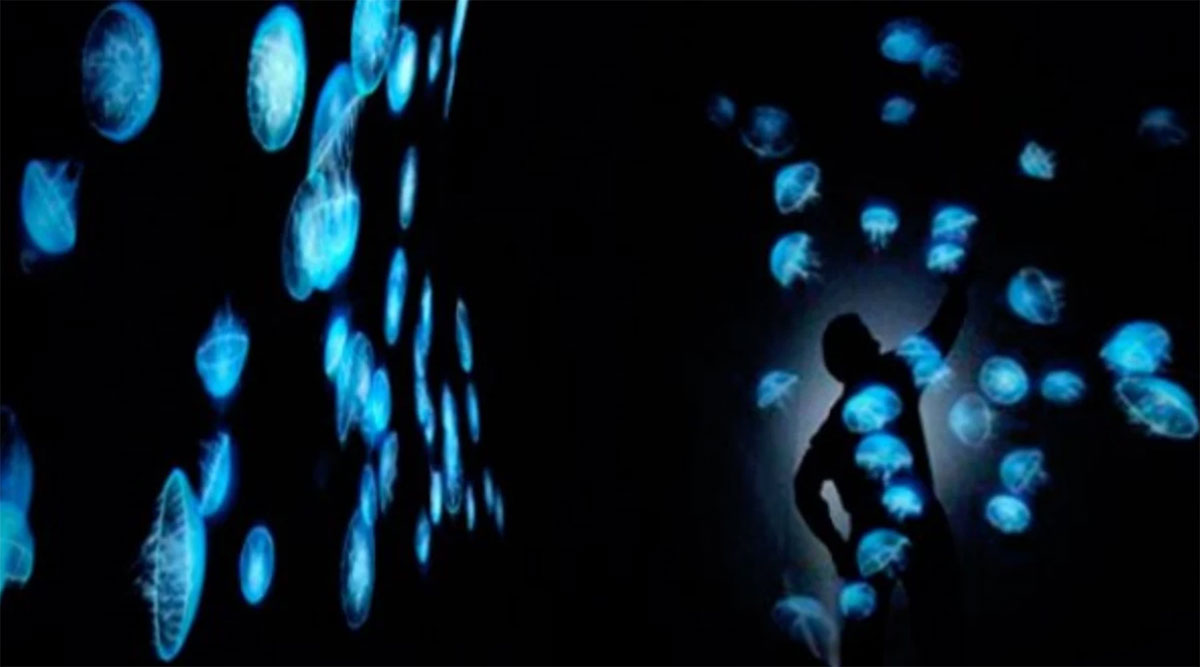
\includegraphics[width=0.8\textwidth]{./04-figuras/takahito_matsuo}
    \label{fig:takahito_matsuo}
\end{figure}
\vspace*{-0,9cm}
{\raggedright \fonte{\citeonline{soares}}}\\

A figura \ref{fig:jim_campbell} mostra o trabalho do artista Jim Campbell que, em um mundo de alta definição e telas cada vez mais finas, usa tecnologia para produzir o contrário: imagens borradas e em baixa resolução em painéis tridimensionais. Essas video-esculturas são compostas por grades de LEDs que atuam como uma televisão de pixels desconstruída. 

\begin{figure}[H]
    \centering
    \caption{Light Topography Wave, Jim Campbell, 2014}
	\vspace*{0,2cm}
    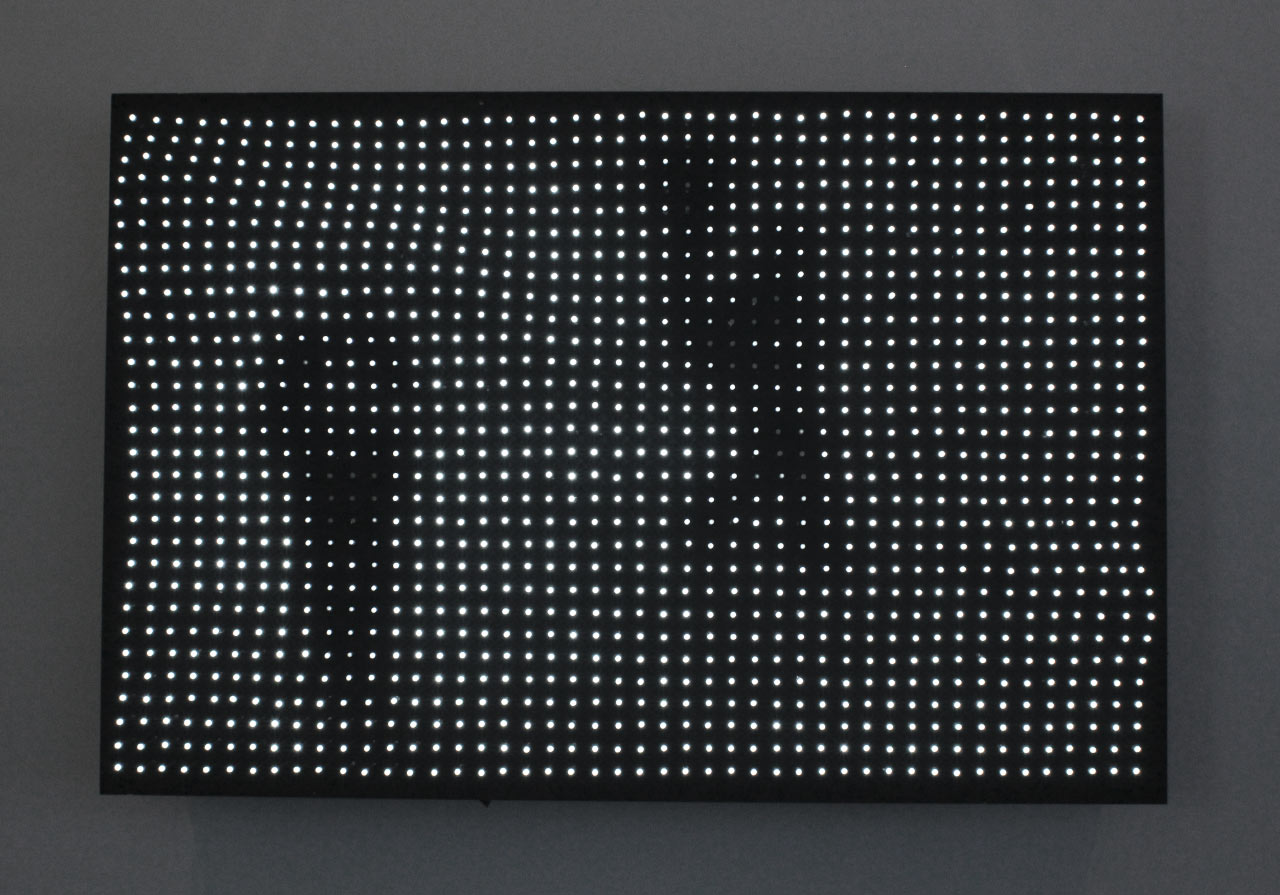
\includegraphics[width=0.8\textwidth]{./04-figuras/jim_campbell}
    \label{fig:jim_campbell}
\end{figure}
\vspace*{-0,9cm}
{\raggedright \fonte{Disponível em: <https://design-milk.com/pixelated-led-art-jim-campbell/>. Acesso em: 22 mar. 2018}}\\

\citeonline[p. 40]{soares}, afirma que "a maioria dos autores que trabalham com arte e tecnologia procuram o espaço do cubo preto como espaço expositivo. Neste espaço o que interessa é um novo ver, um espanto com a imagem". Diz ainda que o nome cubo preto para este tipo de exposição surge em contraposição ao cubo branco, criado por Brian O'Doherty, num ensaio publicado pela revista Artforum em 1976, fazendo alusão ao espaço das galerias de arte, com paredes brancas, sem janelas isolando o espetador num meio aparentemente atemporal. A ideia do cubo preto surge como ambiente ideal para propagação da luz e é também uma forma de imersão no interior da mente do artista.
\index{Cubo Preto}
